\subsection{Elasticity in 1D}
\renewcommand{\arraystretch}{2}
	\begin{tabularx}{ \columnwidth} {lXXX}
		Law & formula &&\\
		Hook's Law & $F = k\cdot \Delta x$ &
		momentum   & $p = m\cdot v$\\
		
		momentum flux & $J_p = \dfrac{\partial p}{\partial t}$&
		momentum flux density & $j_p = \dfrac{J_p}{A}$\\
		
		mechanical stress & $\sigma_{11} = -j_p = \frac{-J_p}{A} $ &
		cutting force & $F = \int_A \sigma_{11} dA$\\
		&&&\\
		
		\textbf{Momentum Balance equation} & $\dfrac{\partial \sigma_{11}}{\partial x} + \rho g= 0$ &
		boundary cond. & $\sigma_{11}(L) = \dfrac{F}{A} \newline u(0) = 0$\\
		
		Displacement Field & $u(x) = \Delta u \cdot \dfrac{x}{l}$ & 
		Material Law & $\epsilon_{11} = \dfrac{\partial u(x)}{\partial x} $\newline $ \sigma_{11} = E\cdot \epsilon_{11}$\\ 
		
	\end{tabularx}
\renewcommand{\arraystretch}{1.2}	
	 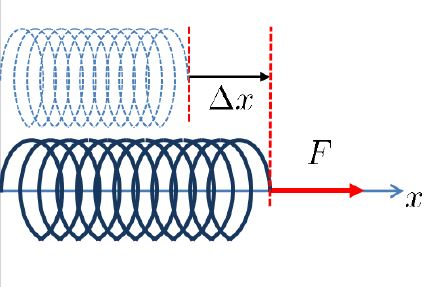
\includegraphics[scale = 0.3]{images/hook}
		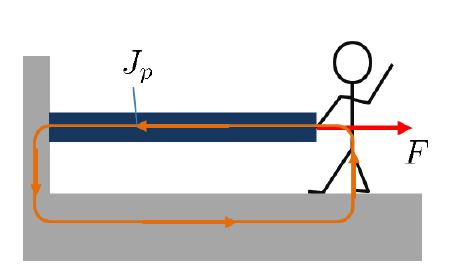
\includegraphics[scale=.3]{images/momentcons}
		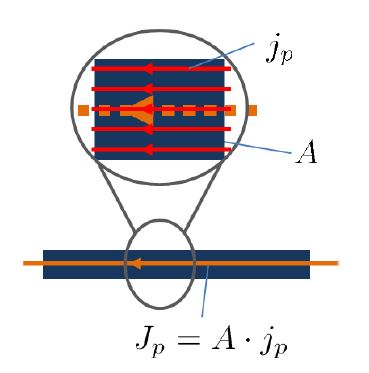
\includegraphics[scale=.3]{images/momflux}
		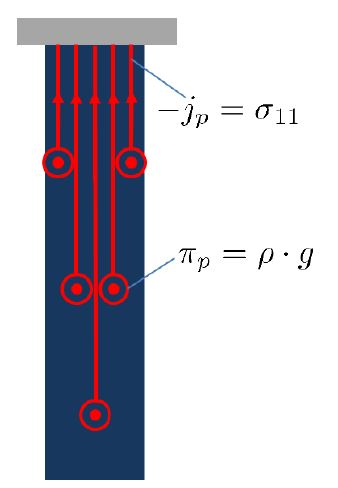
\includegraphics[scale=.3]{images/momfluxdensity}
		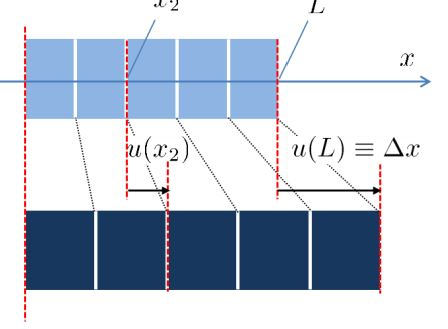
\includegraphics[scale=.3]{images/strain}
%		\includegraphics[scale=.3]{images/}				


\subsection{Elasticity in 3D}
	electrodyamics: scalar charge $q$ $\Rightarrow$ vectorial flux $j$ (0nd rank tensor $\Rightarrow$ 1st rank tensor)
	
	mechanics: vector momentum $\mathbf{p}$ $\Rightarrow$ tensorial flux density $\mathbf{\sigma}$ (1st rank tensor $\Rightarrow$ 2nd rank tensor)

%	$$
%	\sigma = \begin{pmatrix}
%	\sigma_{11} & \sigma_{12} & \sigma_{13} \\
%	\sigma_{21} & \sigma_{22} & \sigma_{23} \\
%	\sigma_{31} & \sigma_{32} & \sigma_{33} 
%	\end{pmatrix}
%	$$
\begin{tabularx}{ \columnwidth} {lXX}
	General momentum balance equation &  $\dfrac{\partial \sigma_{ik}}{\partial x_k} + \rho g_i = 0$ & $\sigma_{ij}$: stress tensor of 2nd rank, characterizes material symmetry: $\sigma_{ij} = \sigma_{ji}$\\
	Cutting Force & $F_i^\alpha = \sigma_{ik} nA^\alpha_k \cdot A^\alpha$ & $\mathbf{n}^\alpha$: normal vector pointing outside of the cuboide\newline $A^\alpha$: face area \\
	Angular Momentum & $\mathbf{M} = 0 $ & \\
	
\end{tabularx}
	\renewcommand{\arraystretch}{2}
\subsection{Special Stress States (Mechanische Spannung $\sigma = F/A$)}
	\begin{tabularx}{\columnwidth}{llXX}
		Stress State & Tensor law & matrix notation & \\ 
		Isotropic Stress State & $\sigma_{ij} = -P\delta_{ik}$&	$ \sigma = \begin{pmatrix} -P & 0 & 0\\ 0 & -P & 0\\ 0 & 0 & -P \end{pmatrix}$ &\vspace*{-1.5cm}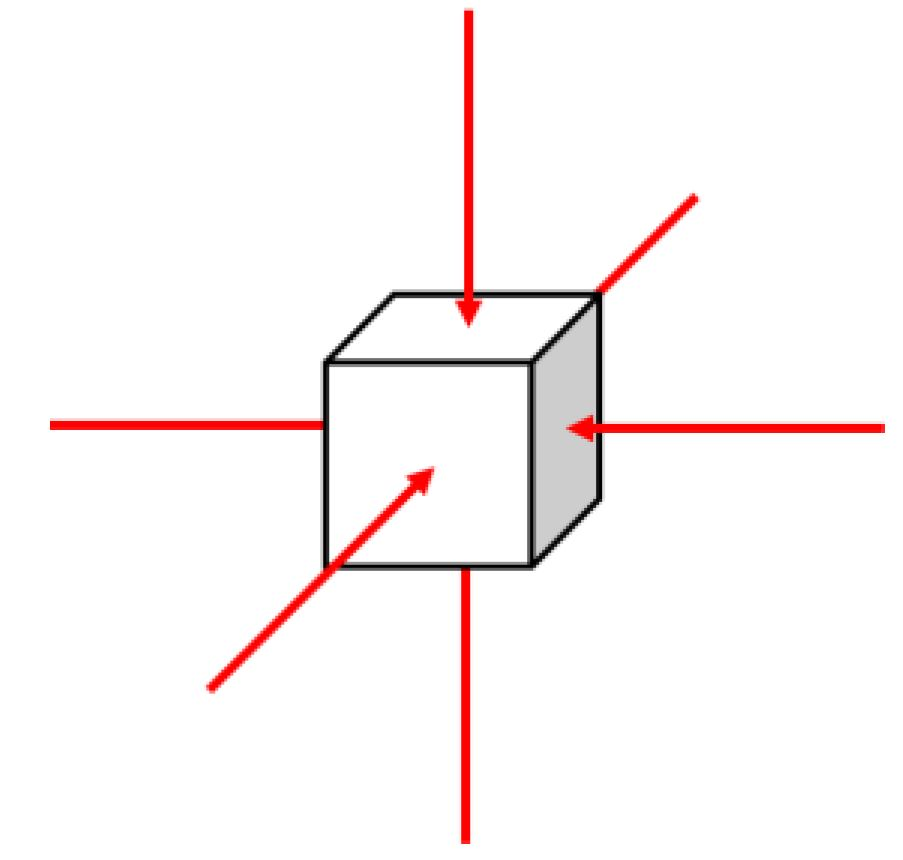
\includegraphics[scale=.2]{images/3Dcfisotropic}\\
		Uniaxial Stress State & & 		$ \sigma = \begin{pmatrix} \sigma_{11} & 0 & 0\\ 0 & 0 & 0\\ 0 & 0 & 0\\ \end{pmatrix}$ &		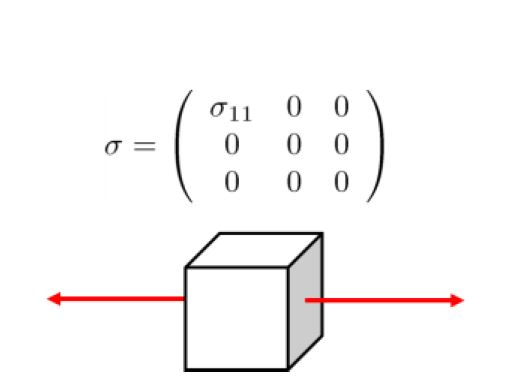
\includegraphics[scale=.3]{images/3Dcfuniaxial}				\\
		Plane Stress State && $ \sigma = \begin{pmatrix} \sigma_{11} & \sigma_{12} & 0\\ \sigma_{21} & \sigma_{22} & 0\\ 0 & 0 & 0\\ \end{pmatrix}$&		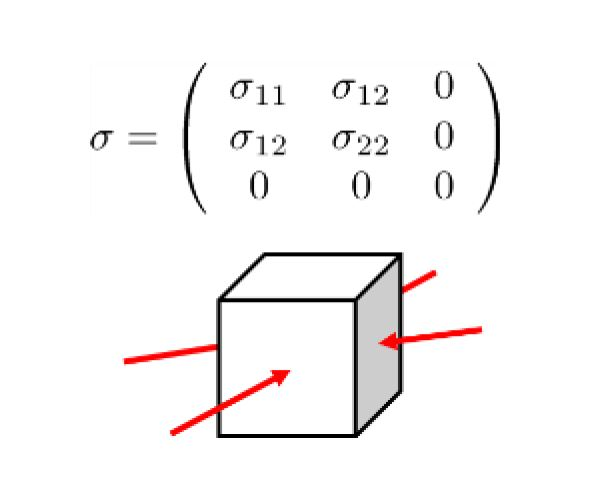
\includegraphics[scale=.3]{images/3Dcfplanestress}				 \\
		Principal Axis Decompensation &&$ \sigma = \begin{pmatrix} \sigma_{11} &  0& 0\\ 0 & \sigma_{22} & 0\\ 0 & 0 & \sigma_{33}\\ \end{pmatrix}$&\\
		Pure Shear Stress State &$\operatorname{tr}\sigma = 0$&$ \sigma = \begin{pmatrix} S &  0& 0\\ 0 & -s & 0\\ 0 & 0 & 0\\ \end{pmatrix}$&		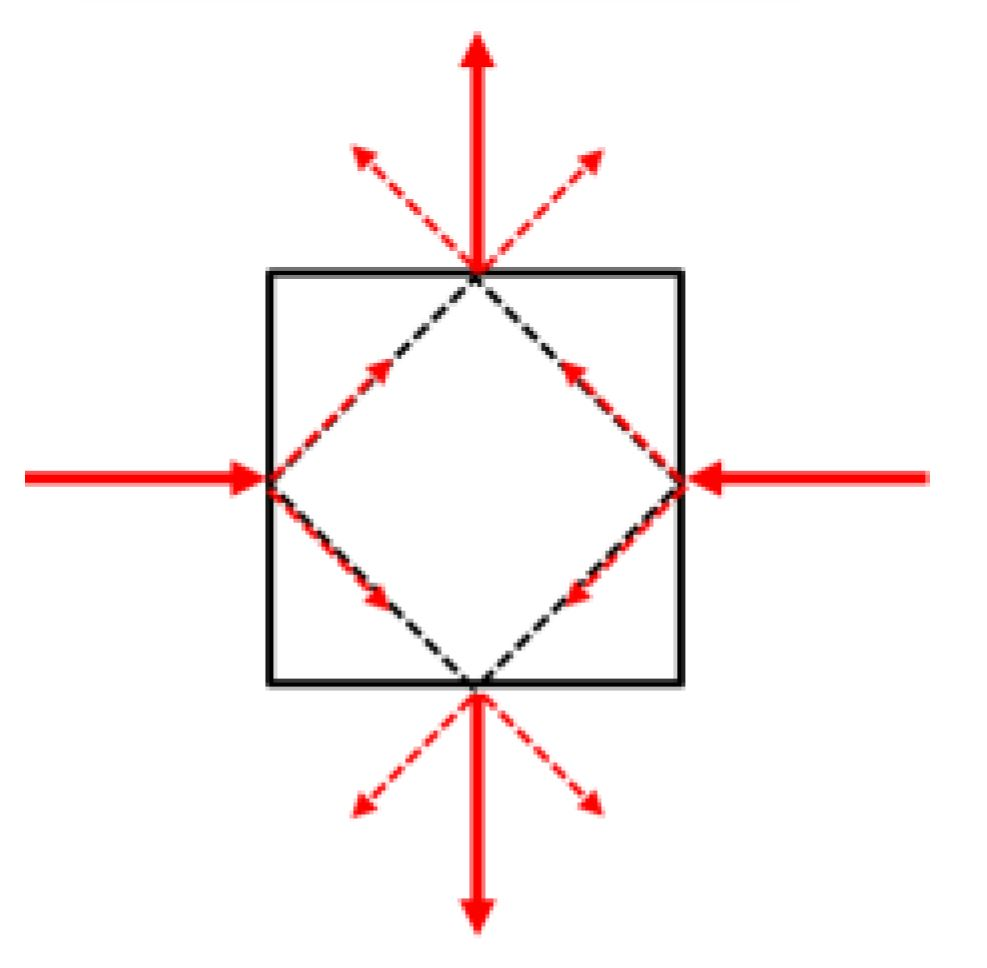
\includegraphics[scale=.3]{images/3Dcfpureshear}				\\
	\end{tabularx}
	\renewcommand{\arraystretch}{1.2}

	\subsubsection{Stress Decomposition (Zerlegung isotropic/shear)}
	\label{stressdecomposition}
	
	$\sigma$ kann in zwei verschiedene Teile zerlegt werden (Tensorverjüngung!!!):
	
	\begin{align}
		\sigma^{iso}=\frac{\operatorname{tr} \sigma}{3} \cdot \mathbf{I} \equiv
		\frac{1}{3} \mathbb{E} : \epsilon
	\end{align}
	
	und
	
	\begin{align}
		\sigma^{shear}= \left(\mathbb{I}- \frac{1}{3}\mathbb{E} \right) : \epsilon
	\end{align}
	
	\textbf{Hint}:
	\begin{align}
		\sigma^{shear} = \sigma -\sigma^{iso}
	\end{align}
	
	
	
	
	
	
	\subsection{Strain Tensors $\epsilon$ (Deformation, Dehnung, Verschiebung)}
	Strain, Dehnung: $\frac{\Delta L}{L}$ (Wirkung die Auftritt durch Stress
	Tensor (Spannung $\frac{F}{A}$) $\sigma$)\\
	Gradient der Deformation: $e = \begin{pmatrix}
	\frac{\partial u_1}{\partial x_1} & \frac{\partial u_1}{\partial x_2} &
	\frac{\partial u_1}{\partial x_3}\\
	\frac{\partial u_2}{\partial x_1} & \frac{\partial u_2}{\partial x_2} &
	\frac{\partial u_2}{\partial x_3}\\
	\frac{\partial u_3}{\partial x_1} & \frac{\partial u_3}{\partial x_2} &
	\frac{\partial u_3}{\partial x_3}\\
	\end{pmatrix}$\\
	Tensor aufteilen (symmetrisch und antisymmetrisch): $e = e^{sym} + e^{anti}$\\
	mechanical strain Tensor: $\epsilon \equiv e^{sym} = \frac{1}{2} (e + e^T) =
	\frac{1}{2} (\frac{\partial u_i}{\partial x_j} + \frac{\partial
		u_j}{\partial x_i})$\\
	Rotational deformation (infinitesimal): $\gamma \equiv e^{anti} = \frac{1}{2} (e
	- e^T)$\\
	Anwendung siehe: Beispiel \ref{9.3} (Seite \pageref{9.3})
	
	\subsubsection{Volume Change of a Deformation}
	$\frac{\Delta V}{V} = tr \epsilon $
	
	\subsubsection{Isotropic Strain (Gestalterhaltend)}
	$\epsilon_{ij} = \epsilon \cdot \delta_{ij} $
	
	\subsubsection{Pure Shear Strain}
	$e_{ij}$ with $trace \epsilon = 0$, Volumen bleibt gleich!
	
	\subsubsection{Strain Decomposition (Zerlegung isotropic/shear)}
	\label{straindecomposition}
	Volumenändernd, isotropic: $\epsilon^{iso} = \frac{tr \epsilon}{3} \cdot \mathbf{I}
	\equiv \frac{1}{3} \mathbb{E} : \epsilon$\\
	
	Volumenerhaltend, shape changing (Formverändernd): $\epsilon^{shear} =
	(\mathbb{I} - \frac{1}{3} \mathbb{E} ) : \epsilon $\\
	\textbf{Hint}: $\epsilon = \epsilon^{iso} + \epsilon^{shear}$ $\rightarrow$
	$\epsilon^{shear} = \epsilon -\epsilon^{iso}$\\
	Wobei (Achtung in Engineering
	Notation siehe Kapitel \ref{tensor4th} auf Seite \pageref{tensor4th}):\\ $ \mathbb{I}^{eng}=
	\begin{pmatrix}
	1 & 0 & 0 & 0 & 0 & 0 \\ 
	0 & 1 & 0 & 0 & 0 & 0 \\ 
	0 & 0 & 1 & 0 & 0 & 0 \\ 
	0 & 0 & 0 & \frac{1}{2} & 0 & 0 \\ 
	0 & 0 & 0 & 0 & \frac{1}{2} & 0 \\ 
	0 & 0 & 0 & 0 & 0 & \frac{1}{2}
	\end{pmatrix} 
	$ und 
	$ \mathbb{E}^{eng}=
	\begin{pmatrix}
	1 & 1 & 1 & 0 & 0 & 0 \\ 
	1 & 1 & 1 & 0 & 0 & 0 \\ 
	1 & 1 & 1 & 0 & 0 & 0 \\ 
	0 & 0 & 0 & 0 & 0 & 0 \\ 
	0 & 0 & 0 & 0 & 0 & 0 \\ 
	0 & 0 & 0 & 0 & 0 & 0
	\end{pmatrix} 
	$
	
	\subsubsection{Plane Strain}
	Plain strain: $\epsilon_{33} = \epsilon_{13} = \epsilon_{23}= 0$ => $\epsilon =
	\begin{pmatrix}
	* & * & 0\\
	* & * & 0\\
	* & * & 0\\
	\end{pmatrix} $\\
	\begin{itemize}
		\item Keine Deformation in z-Achse
		\item Beispiel: Druckstaudamm in Schweizer Alpen (large extension along
		z-axis)
	\end{itemize}
	
	\subsection{Elasticity Tensor E and $\nu$}
	\begin{align}
		\mathbb{C}^{eng} = \frac{E}{1 + \nu} \cdot \begin{pmatrix}
			\frac{1-\nu}{1-2\nu} & \frac{\nu}{1-2\nu} & \frac{\nu}{1-2\nu} & 0 & 0 & 0\\
			\frac{\nu}{1-2\nu} & \frac{1-\nu}{1-2\nu} & \frac{\nu}{1-2\nu} & 0 & 0 & 0\\
			\frac{\nu}{1-2\nu} & \frac{\nu}{1-2\nu} & \frac{1-\nu}{1-2\nu} & 0 & 0 & 0\\
			0 & 0 & 0 & \frac{1}{2} & 0 & 0\\
			0 & 0 & 0 & 0 & \frac{1}{2} & 0\\
			0 & 0 & 0 & 0 & 0 & \frac{1}{2}\\
		\end{pmatrix}
	\end{align}
	Vereinfacht (wohl ohne Scherung):
	\begin{align}\label{eq:elasticity}
		\mathbf{C} = \frac{E}{1 + \nu} \cdot \begin{pmatrix}
			\frac{1-\nu}{1-2\nu} & \frac{\nu}{1-2\nu} & \frac{\nu}{1-2\nu}\\
			\frac{\nu}{1-2\nu} & \frac{1-\nu}{1-2\nu} & \frac{\nu}{1-2\nu}\\
			\frac{\nu}{1-2\nu} & \frac{\nu}{1-2\nu} & \frac{1-\nu}{1-2\nu}
		\end{pmatrix}
	\end{align}
	
	E-module (Young's modulus): $E$\\
	Poisson's ratio: $\nu$\\
	
	\textbf{Elasticity Tensor in Plane Strain $\epsilon$}\\
	$\mathbb{C}^{eng} = \frac{E}{1 + \nu} \cdot \begin{pmatrix}
	\frac{1-\nu}{1-2\nu} & \frac{\nu}{1-2\nu} & 0\\
	\frac{\nu}{1-2\nu} & \frac{1-\nu}{1-2\nu} & 0\\
	0 & 0 & \frac{1}{2}
	\end{pmatrix}$\\
	
	\textbf{Elasticity Tensor in Plane Stress $\sigma$}\\
	$\mathbb{C}^{eng} = \frac{E}{1 + \nu} \cdot \begin{pmatrix}
	\frac{1}{1-\nu} & \frac{\nu}{1-\nu} & 0\\
	\frac{\nu}{1-\nu} & \frac{1}{1-\nu} & 0\\
	0 & 0 & \frac{1}{2}
	\end{pmatrix}$\\
	
	\subsection{Kompressionsmodul K / Schermodul G}
	
	Kompressionsmodul (bulk modulus) $K$\\
	
	Schermodul (shear modulus) $G$\\
	
	\textbf{Isotropic Mechanical Material Laws (Skript 8.2)}\\
	
	
	\begin{align}\label{eq:materiallaw}
		\mathbb{C}^{iso} = K \cdot \mathbb{E} + 2G \cdot (\mathbb{I} - \frac{1}{3}
		\mathbb{E})
	\end{align}
	etwas umgeformt:
	\begin{align}
		\mathbb{C}^{iso} = (K - \frac{2}{3} G) \cdot \mathbb{E} + 2G \cdot \mathbb{I}
	\end{align}
	
	Formel \ref{eq:materiallaw} in Voigt's Notation:
	\begin{align}
		\mathbb{C}^{eng} = K \cdot \begin{pmatrix}
			1 & 1 & 1 & 0 & 0 & 0\\
			1 & 1 & 1 & 0 & 0 & 0\\
			1 & 1 & 1 & 0 & 0 & 0\\
			0 & 0 & 0 & 0 & 0 & 0\\
			0 & 0 & 0 & 0 & 0 & 0\\
			0 & 0 & 0 & 0 & 0 & 0\\
		\end{pmatrix}
		+ 2 G \cdot \begin{pmatrix}
			\frac{2}{3} & -\frac{1}{3} & -\frac{1}{3} & 0 & 0 & 0\\
			-\frac{1}{3} & \frac{2}{3} & -\frac{1}{3} & 0 & 0 & 0\\
			-\frac{1}{3} & -\frac{1}{3} & \frac{2}{3} & 0 & 0 & 0\\
			0 & 0 & 0 & \frac{1}{2} & 0 & 0\\
			0 & 0 & 0 & 0 & \frac{1}{2} & 0\\
			0 & 0 & 0 & 0 & 0 & \frac{1}{2}\\
		\end{pmatrix}
	\end{align}
	
	\textbf{Deformation under Uniaxial Stress}\\
	\begin{align}
		\begin{pmatrix}
			\sigma_{11}\\
			0\\
			0
		\end{pmatrix} = 
		\begin{pmatrix}
			K + \frac{4G}{3} & K - \frac{2G}{3} & K - \frac{2G}{3}\\
			K - \frac{2G}{3} & K + \frac{4G}{3} & K - \frac{2G}{3}\\
			K - \frac{2G}{3} & K - \frac{2G}{3} & K + \frac{4G}{3}\\
		\end{pmatrix} =
		\begin{pmatrix}
			\epsilon_{11}\\
			- \epsilon_{22}\\
			- \epsilon_{33}
		\end{pmatrix}
	\end{align}
	
	Repräsentiert:
	\begin{align}
		\sigma_{11} = E \cdot \epsilon_{11}
	\end{align}
	Gleichungssystem nach E aufgelöst:
	\begin{align}
		E \equiv \frac{9 K G}{3K + G}
	\end{align}
	
\newpage



		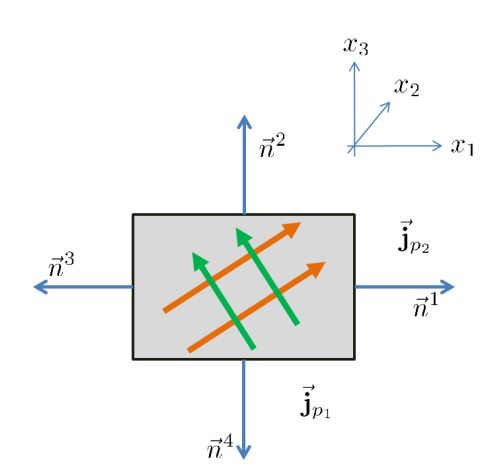
\includegraphics[scale=.3]{images/3Dmomentum}				
		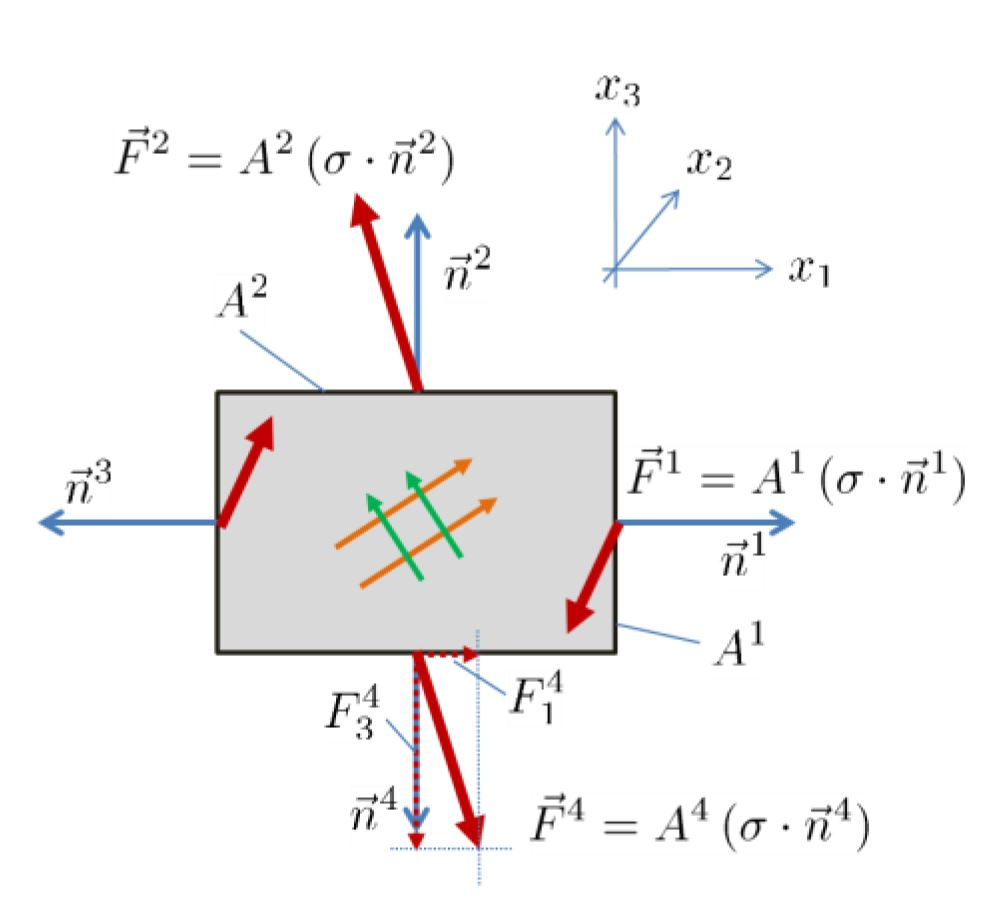
\includegraphics[scale=.3]{images/3Dcuttingforces}				
		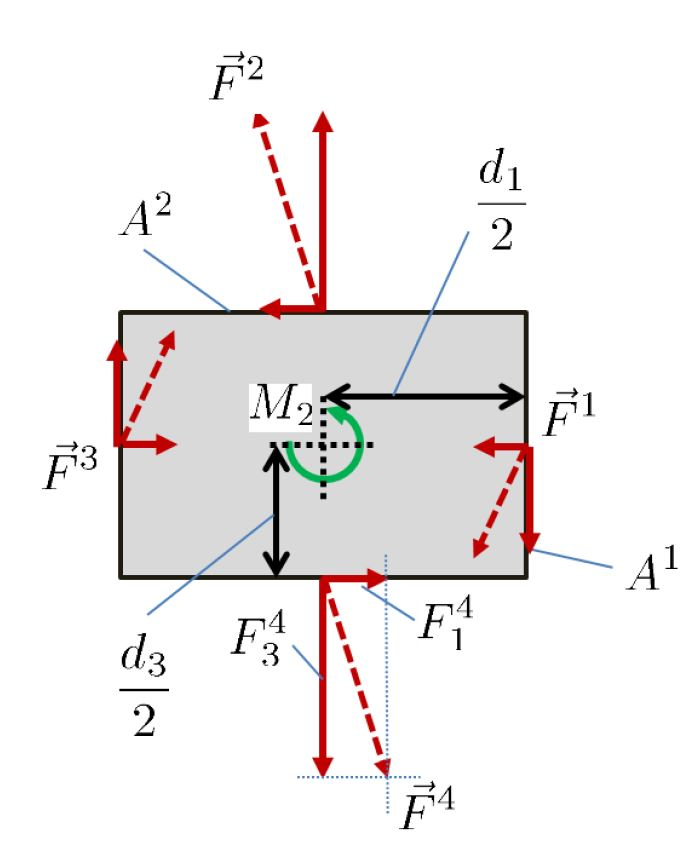
\includegraphics[scale=.3]{images/3Dangularmomentum}				
		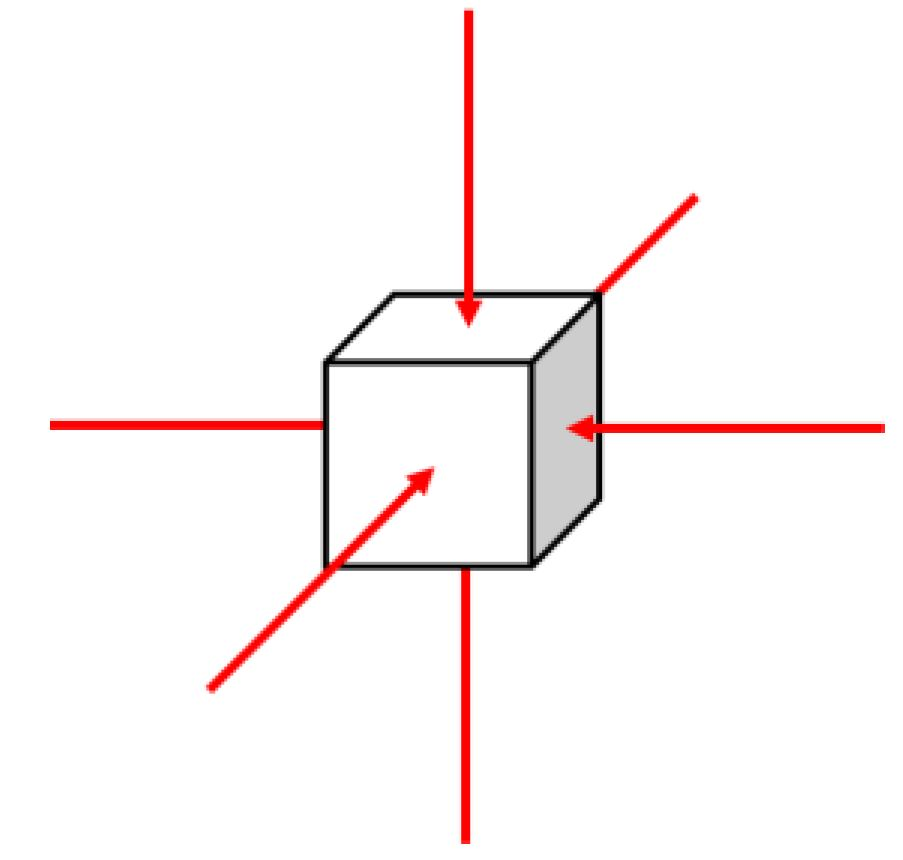
\includegraphics[scale=.3]{images/3Dcfisotropic}				
		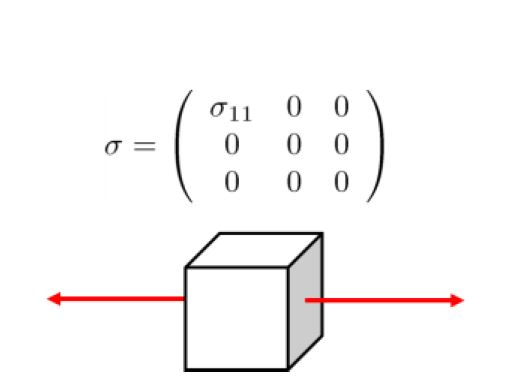
\includegraphics[scale=.3]{images/3Dcfuniaxial}				
		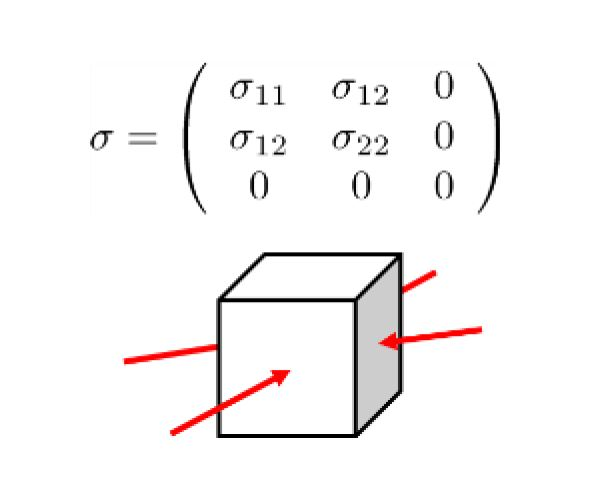
\includegraphics[scale=.3]{images/3Dcfplanestress}				
		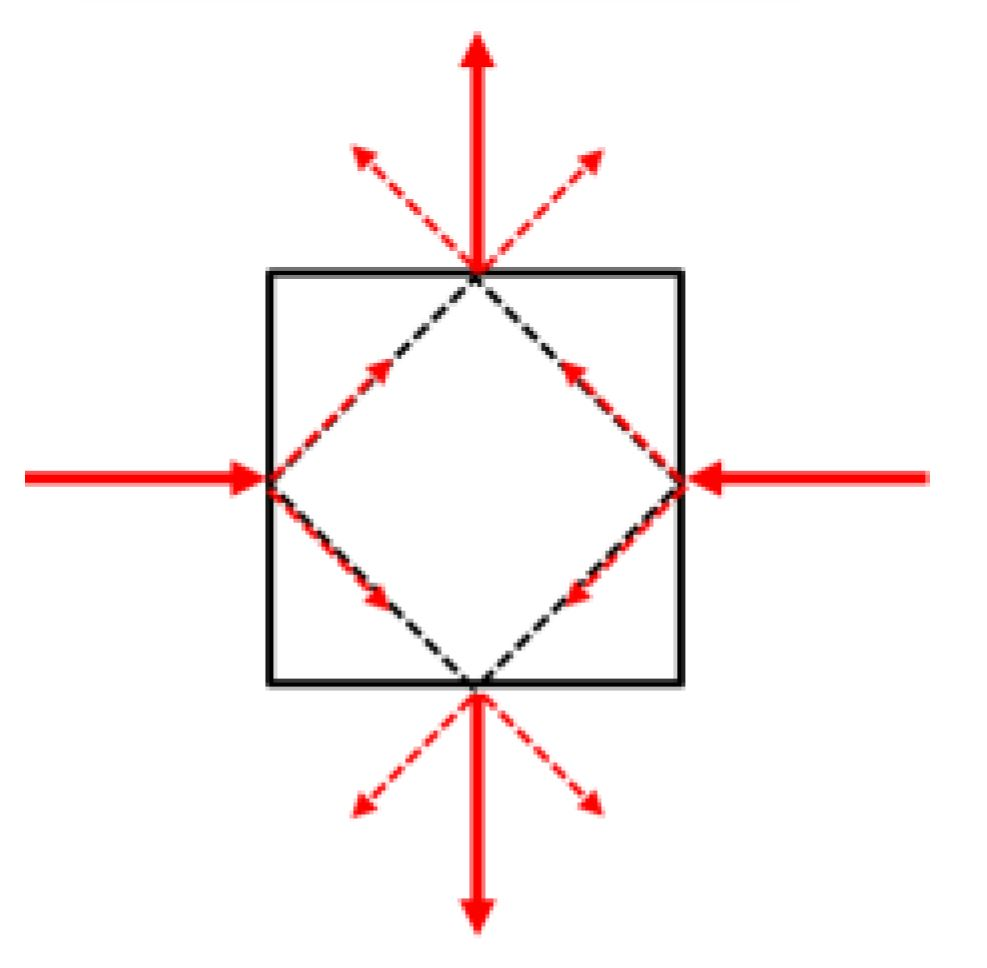
\includegraphics[scale=.3]{images/3Dcfpureshear}				
		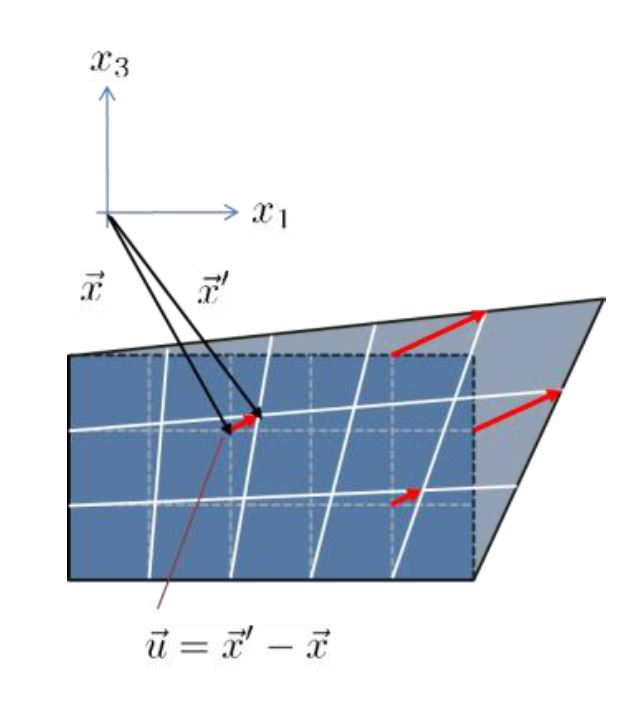
\includegraphics[scale=.3]{images/2Ddeformation}				
		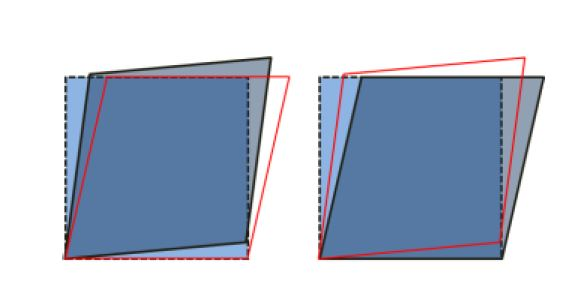
\includegraphics[scale=.3]{images/deformgrad}
		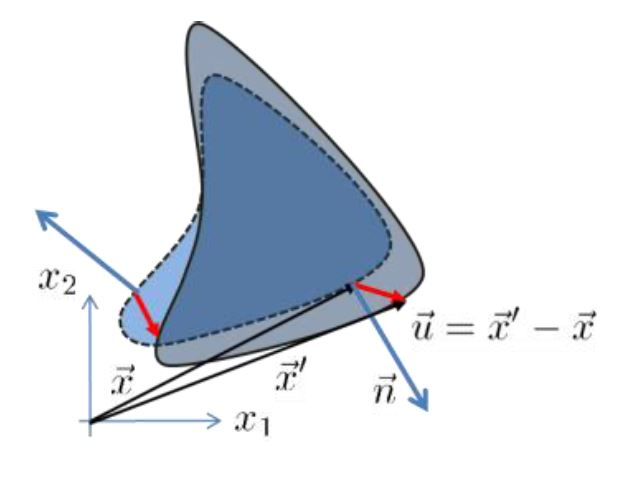
\includegraphics[scale=.3]{images/deformvolume}
		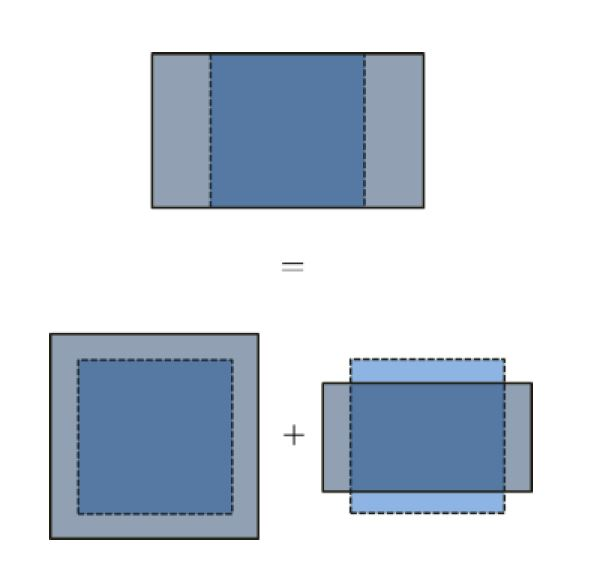
\includegraphics[scale=.3]{images/allstates}
%		\includegraphics[scale=.3]{images/}



